\documentclass[10pt, xcolor=table]{beamer}

\setbeamertemplate{note page}[default]
%\setbeameroption{hide notes}
\setbeameroption{show notes}
\setbeamerfont{footnote}{size=\tiny}

\usetheme[progressbar=frametitle]{metropolis}
\usepackage{appendixnumberbeamer}

\usepackage{booktabs}
\usepackage[scale=2]{ccicons}

\usepackage{pgfplots}
\usepgfplotslibrary{dateplot}
\usepackage{multicol}
\setlength{\columnsep}{1.5cm}



\usepackage{animate}
\usepackage{lmodern}
\usepackage[T1]{fontenc}
\usepackage{mathtools}
\usepackage{graphicx}
\usepackage{caption}
\usepackage{tikz}
\usetikzlibrary{positioning}


\definecolor{set1}{RGB}{228, 26, 28}
\definecolor{set2}{RGB}{77, 175, 74}
\definecolor{set3}{RGB}{255, 127, 0}
\definecolor{set4}{RGB}{166, 86, 40}
\definecolor{set5}{RGB}{153, 153, 153}

\usepackage{xspace}
\newcommand{\themename}{\textbf{\textsc{metropolis}}\xspace}

\newcommand\Fontvi{\fontsize{8}{9}\selectfont}
\newcommand\Fontvr{\fontsize{6}{7}\selectfont}

\setbeamerfont{parent A}{size=\small}

%\usepackage[table]{xcolor} 


\title{Digital Transformation of Healthcare}
\subtitle{Evaluating Predictions}
% \date{\today}
\date{}
\author{Michoel Snow, MD PhD, Glen Ferguson, PhD}
\institute{Center for Health Data Innovations}
% \titlegraphic{\hfill\includegraphics[height=1.5cm]{logo.pdf}}

\begin{document}

\maketitle


\begin{frame}{Objectives}
	After this lecture students will be able to 
	\begin{itemize}
		\item Distinguish between classification and regression metrics
		\item Compare and contrast the use of different metrics to evaluate predictions
		\item 
	\end{itemize}%
\end{frame}


\begin{frame}
	\begin{center}
		\Large{Metrics for Evaluation of Classification Models}
	\end{center}
\end{frame}	


\begin{frame}{Confusion Matrix}
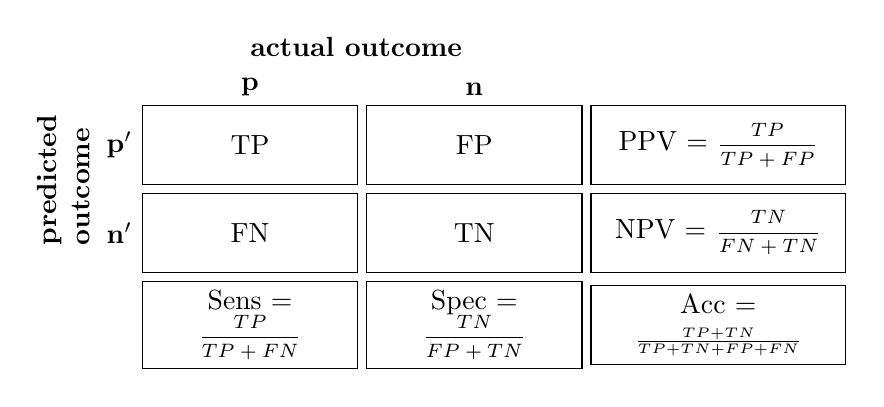
\begin{tikzpicture}[ampersand replacement=\&,
box/.style={draw,rectangle,minimum size=1cm,text width=2.5cm,align=center},
box2/.style={draw,rectangle,minimum size=1cm,text width=3cm,align=center}]
\matrix (conmat) [row sep=.1cm,column sep=.1cm] {
\node (tpos) [box,
    label=left:\( \mathbf{p'} \),
    label=above:\( \mathbf{p} \),
    ] {TP};
\&
\node (fpos) [box,
    label=above:\textbf{n}] {FP};
\&
\node (ppv) [box2] {PPV = \scriptsize{$\dfrac{TP}{TP+FP}$}};
\\
\node (fneg) [box,
    label=left:\( \mathbf{n'} \)] {FN};
\&
\node (tneg) [box] {TN};
\&
\node (npv) [box2] {NPV = \scriptsize{$\dfrac{TN}{FN+TN}$}};
\\
\node (sens) [box] {Sens = \scriptsize{$\dfrac{TP}{TP+FN}$}};
\&
\node (spec) [box] {Spec = \scriptsize{$\dfrac{TN}{FP+TN}$}};
\&
\node (acc) [box2] {Acc = \scriptsize{$\frac{TP+TN}{TP+TN+FP+FN}$}};
%\node (f1) [box2] {F1 = \scriptsize{$\dfrac{2 \times Sens \times PPV}{PPV + Sens}$}};
\\
};
\node [rotate=90, anchor=center,xshift=.35cm, left=1cm of tpos, text width=1.5cm,align=center ] {\textbf{predicted \\ outcome}};
\node [above=0.5cm of fpos,xshift=-1.5cm,align=left] {\textbf{actual outcome}};
\end{tikzpicture}
\end{frame}

%F1 &= \frac{2 \times Sens \times PPV}{Sens + PPV} \\

\begin{frame}{Confusion Matrix}
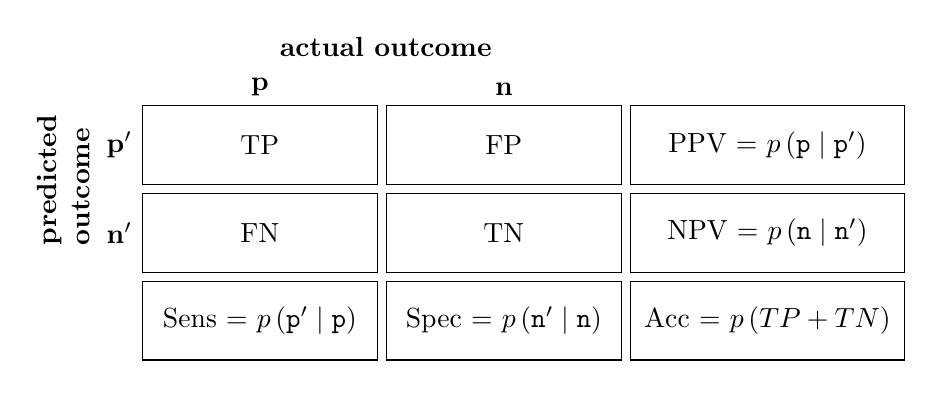
\begin{tikzpicture}[ampersand replacement=\&,
box/.style={draw,rectangle,minimum size=1cm,text width=2.75cm,align=center},
box2/.style={draw,rectangle,minimum size=1cm,text width=3.25cm,align=center}]
\matrix (conmat) [row sep=.1cm,column sep=.1cm] {
\node (tpos) [box,
    label=left:\( \mathbf{p'} \),
    label=above:\( \mathbf{p} \),
    ] {TP};
\&
\node (fpos) [box,
    label=above:\textbf{n}] {FP};
\&
\node (ppv) [box2] {PPV = {$p\left(\texttt{\textbf{p}}\mid \texttt{\textbf{p}}'\right)$}};
\\
\node (fneg) [box,
    label=left:\( \mathbf{n'} \)] {FN};
\&
\node (tneg) [box] {TN};
\&
\node (npv) [box2] {NPV = {$p\left(\texttt{\textbf{n}}\mid \texttt{\textbf{n}}'\right)$}};
\\
\node (sens) [box] {Sens = {$p\left(\texttt{\textbf{p}}'\mid \texttt{\textbf{p}}\right)$}};
\&
\node (spec) [box] {Spec = {$p\left(\texttt{\textbf{n}}'\mid \texttt{\textbf{n}}\right)$}};
\&
\node (acc) [box2] {Acc = {$p\left(TP + TN\right)$}};
\\
};
\node [rotate=90, anchor=center,xshift=.35cm, left=1cm of tpos, text width=1.5cm,align=center ] {\textbf{predicted \\ outcome}};
\node [above=0.5cm of fpos,xshift=-1.5cm,align=left] {\textbf{actual outcome}};
\end{tikzpicture}

\end{frame}




\begin{frame}{Confusion Matrix}
\vspace{4em}
\begin{center}
\begin{tikzpicture}[transform canvas={scale=0.75}, ampersand replacement=\&,
box/.style={draw,rectangle,minimum size=1cm,text width=2.75cm,align=center},
box2/.style={draw,rectangle,minimum size=1cm,text width=3.25cm,align=center}]
\matrix (conmat) [row sep=.1cm,column sep=.1cm] {
\node (tpos) [box,
    label=left:\( \mathbf{p'} \),
    label=above:\( \mathbf{p} \),
    ] {TP};
\&
\node (fpos) [box,
    label=above:\textbf{n}] {FP};
\&
\node (ppv) [box2] {PPV = {$p\left(\texttt{\textbf{p}}\mid \texttt{\textbf{p}}'\right)$}};
\\
\node (fneg) [box,
    label=left:\( \mathbf{n'} \)] {FN};
\&
\node (tneg) [box] {TN};
\&
\node (npv) [box2] {NPV = {$p\left(\texttt{\textbf{n}}\mid \texttt{\textbf{n}}'\right)$}};
\\
\node (sens) [box] {Sens = {$p\left(\texttt{\textbf{p}}'\mid \texttt{\textbf{p}}\right)$}};
\&
\node (spec) [box] {Spec = {$p\left(\texttt{\textbf{n}}'\mid \texttt{\textbf{n}}\right)$}};
\&
\node (acc) [box2] {Acc = {$p\left(TP + TN\right)$}};
%\node (f1) [box2] {F1 = \scriptsize{$\dfrac{2 \times Sens \times PPV}{PPV + Sens}$}};
\\
};
\node [rotate=90, anchor=center,xshift=.35cm, left=1cm of tpos, text width=1.5cm,align=center ] {\textbf{predicted \\ outcome}};
\node [above=0.5cm of fpos,xshift=-1.5cm,align=left] {\textbf{actual outcome}};
\end{tikzpicture}
\end{center}
\vspace{3em}

\begin{table}
	\scriptsize
	\begin{tabular}{c c c}
		Parameter & Interpretation & Inappropriate for \\ \hline \hline
		Accuracy & Overall proximity of test to reality & Imbalanced sample sizes \\	
		Sensitivity  &  & \\ 
		Specificity  &  & \\
		PPV  &  &  \\
		NPV &  &  \\
	\end{tabular}
\end{table}
\end{frame}













\begin{frame}{Confusion Matrix}
\vspace{4em}
\begin{center}
\begin{tikzpicture}[transform canvas={scale=0.75}, ampersand replacement=\&,
box/.style={draw,rectangle,minimum size=1cm,text width=2.75cm,align=center},
box2/.style={draw,rectangle,minimum size=1cm,text width=3.25cm,align=center}]
\matrix (conmat) [row sep=.1cm,column sep=.1cm] {
\node (tpos) [box,
    label=left:\( \mathbf{p'} \),
    label=above:\( \mathbf{p} \),
    ] {TP};
\&
\node (fpos) [box,
    label=above:\textbf{n}] {FP};
\&
\node (ppv) [box2] {PPV = {$p\left(\texttt{\textbf{p}}\mid \texttt{\textbf{p}}'\right)$}};
\\
\node (fneg) [box,
    label=left:\( \mathbf{n'} \)] {FN};
\&
\node (tneg) [box] {TN};
\&
\node (npv) [box2] {NPV = {$p\left(\texttt{\textbf{n}}\mid \texttt{\textbf{n}}'\right)$}};
\\
\node (sens) [box] {Sens = {$p\left(\texttt{\textbf{p}}'\mid \texttt{\textbf{p}}\right)$}};
\&
\node (spec) [box] {Spec = {$p\left(\texttt{\textbf{n}}'\mid \texttt{\textbf{n}}\right)$}};
\&
\node (acc) [box2] {Acc = {$p\left(TP + TN\right)$}};
%\node (f1) [box2] {F1 = \scriptsize{$\dfrac{2 \times Sens \times PPV}{PPV + Sens}$}};
\\
};
\node [rotate=90, anchor=center,xshift=.35cm, left=1cm of tpos, text width=1.5cm,align=center ] {\textbf{predicted \\ outcome}};
\node [above=0.5cm of fpos,xshift=-1.5cm,align=left] {\textbf{actual outcome}};
\end{tikzpicture}
\end{center}
\vspace{3em}

\begin{table}
	\scriptsize
	\begin{tabular}{c c c}
		Parameter & Interpretation & Inappropriate for \\ \hline \hline
		Accuracy & Overall proximity of test to reality & Imbalanced sample sizes \\	
		Sensitivity  & Chance of a false negative &  Expensive testing/Mild disease\\ 
		Specificity  & Chance of a false positive &  Cheap testing/Severe disease\\
		PPV  & Sensitivity diagnostic utility & Very high prevalence \\
		NPV & Specificity diagnostic utility & Very low prevalence \\
	\end{tabular}
\end{table}
\end{frame}



%
%\begin{frame}{Confusion Matrix}
%\vspace{4em}
%\begin{center}
%\begin{tikzpicture}[transform canvas={scale=0.75}, ampersand replacement=\&,
%box/.style={draw,rectangle,minimum size=1cm,text width=2.75cm,align=center},
%box2/.style={draw,rectangle,minimum size=1cm,text width=3cm,align=center}]
%\matrix (conmat) [row sep=.1cm,column sep=.1cm] {
%\node (tpos) [box,
%    label=left:\( \mathbf{p'} \),
%    label=above:\( \mathbf{p} \),
%    ] {TP};
%\&
%\node (fpos) [box,
%    label=above:\textbf{n}] {FP};
%\&
%\node (ppv) [box2] {PPV = {$p\left(\texttt{\textbf{p}}\mid \texttt{\textbf{p}}'\right)$}};
%\\
%\node (fneg) [box,
%    label=left:\( \mathbf{n'} \)] {FN};
%\&
%\node (tneg) [box] {TN};
%\&
%\node (npv) [box2] {NPV = {$p\left(\texttt{\textbf{n}}\mid \texttt{\textbf{n}}'\right)$}};
%\\
%\node (sens) [box] {Sens = {$p\left(\texttt{\textbf{p}}'\mid \texttt{\textbf{p}}\right)$}};
%\&
%\node (spec) [box] {Spec = {$p\left(\texttt{\textbf{n}}'\mid \texttt{\textbf{n}}\right)$}};
%\&
%\node (acc) [box2] {Acc = {$p\left(TP + TN\right)$}};
%%\node (f1) [box2] {F1 = \scriptsize{$\dfrac{2 \times Sens \times PPV}{PPV + Sens}$}};
%\\
%};
%\node [rotate=90, anchor=center,xshift=.35cm, left=1cm of tpos, text width=1.5cm,align=center ] {\textbf{predicted \\ outcome}};
%\node [above=0.5cm of fpos,xshift=-1.5cm,align=left] {\textbf{actual outcome}};
%\end{tikzpicture}
%\end{center}
%\vspace{3em}
%
%\begin{table}
%	\scriptsize
%	\begin{tabular}{c c c}
%	Condition & Stats & Example \\ \hline \hline
%	High Sensitivity, Low Specificity & \textbf{p}$'$ $>>$ \textbf{n}$'$ & test is always  positive \\	
%	Low Sensitivity, High Specificity  & \textbf{n}$'$ $>>$ \textbf{p}$'$ & test is always negative \\
%	High PPV, Low NPV & \textbf{p} $>>$ \textbf{n} & high disease prevalence \\
%	Low PPV, High NPV & \textbf{n} $>>$ \textbf{p} & low disease prevalence \\
%	High PPV, Low Sensitivity & FN $>>$ FP & say they are negative most of the time for a high prevalence disease \\
%	High Sensitivity, Low NPV & & \\
%	High Specificity, Low NPV & & \\
%	High PPV, Low Specificity & & \\
%	\end{tabular}
%\end{table}
%
%\end{tabular}
%\end{frame}

\begin{frame}{Combined Statistics}

\begin{table}
	\scriptsize
	\begin{tabular}{c c c}
		Function of & Metric & Formula\\ \hline \hline \\ 
		Sensitivity, Specificity  & Positive Likelihood Ratio/ROC & $\dfrac{sensitivity}{1-specificity}$ \\ [1.5em]
		Sensitivity, Specificity  & Negative Likelihood Ratio & $\dfrac{1-sensitivity}{specificity}$ \\ [1.5em]
		Sensitivity, PPV & F1 score & $\dfrac{2}{\dfrac{1}{sensitivity} + \dfrac{1}{PPV} }$  \\ [4em]
		TP, TN, FP, FN & Matthews correlation coefficient & \tiny{$\dfrac{TP\times TN-FP\times FN}{\sqrt{\left(TP + FP\right)\left(TP+FN\right)\left(TN+FP\right)\left(TN+FN\right)}}$} \\
	\end{tabular}
\end{table}
\end{frame}


\begin{frame}{Likelihood Ratios}
	\begin{center}
		Does a test result change the probability that a person has a certain condition?
	\end{center}
	\begin{align*}
		LR+ &= \dfrac{sensitivity}{1 - specificity} = \dfrac{P\left(T+ \mid D+\right)}{P\left(T+ \mid D-\right)} \\[1.5em]
		LR- &= \dfrac{1 - sensitivity}{specificity} = \dfrac{P\left(T- \mid D+\right)}{P\left(T- \mid D-\right)}
	\end{align*}
%	\begin{center}
%		
%	\end{center}
\end{frame}

\begin{frame}{Likelihood Ratios}
	\begin{center}
		\rowcolors{2}{gray!25}{white}
		\begin{tabular}{c c}
			\rowcolor{gray!50}
			Likelihood Ratio & Approximate Change in Probability(\%) \\ \hline
			0.1 & -45 \\
			0.2 & -30 \\
			0.5 & -15 \\
			1 & 0 \\
			2 & +15 \\
			5 & +30 \\
			10 & +45
		\end{tabular} \\[2em]
		Change in post test probability $\approx 0.2 \times \ln{LR}$ \footnote{{McGee, Steven. "Simplifying likelihood ratios." Journal of general internal medicine 17.8 (2002): 647-650.
APA	
}}
	\end{center}
\end{frame}


\begin{frame}{Hypothesis Testing}
	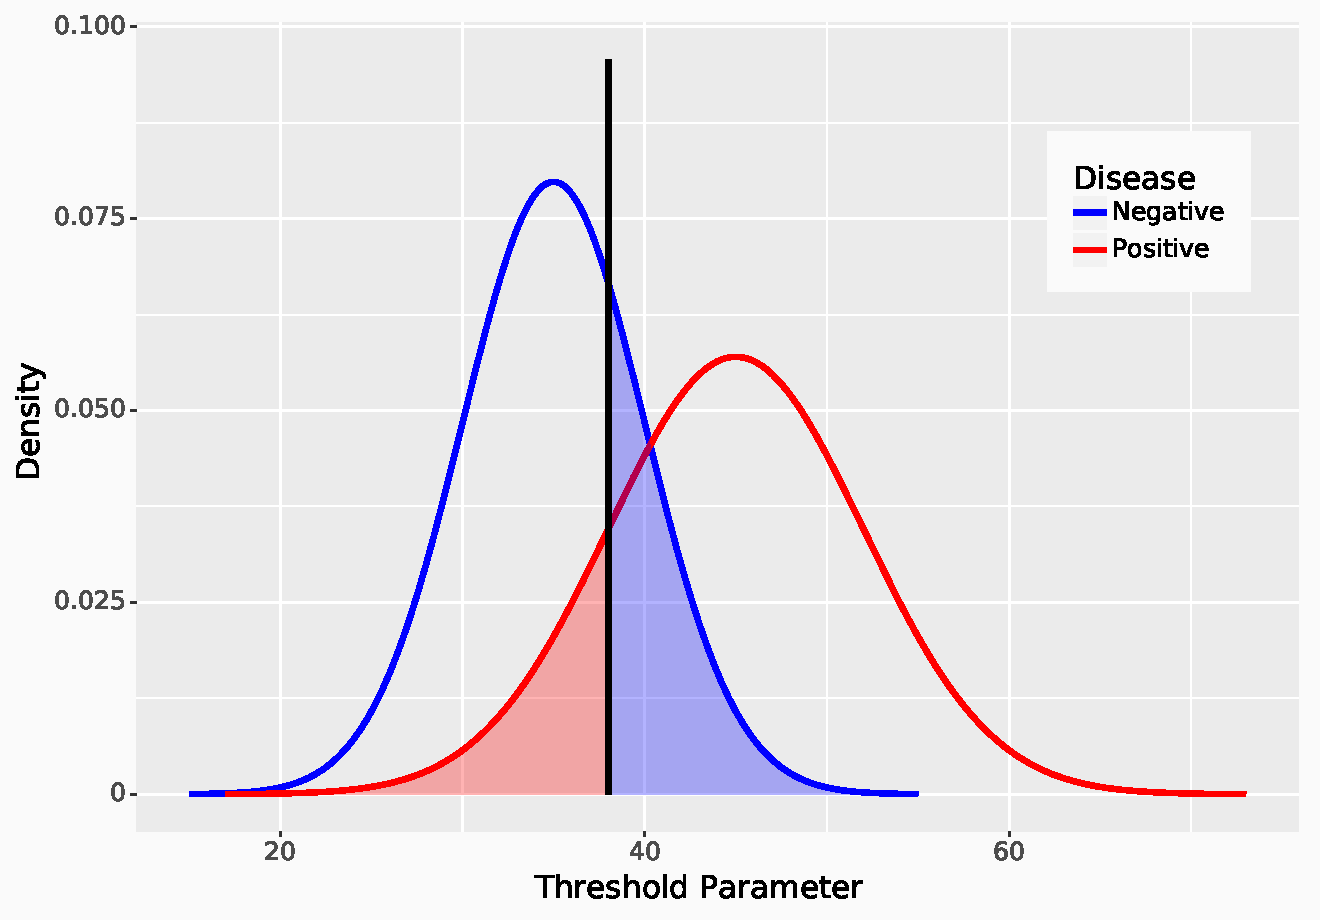
\includegraphics[height=0.8\textheight]{images/overlap_distr.pdf}
\end{frame}


\begin{frame}{Hypothesis Testing}
	\begin{center}
		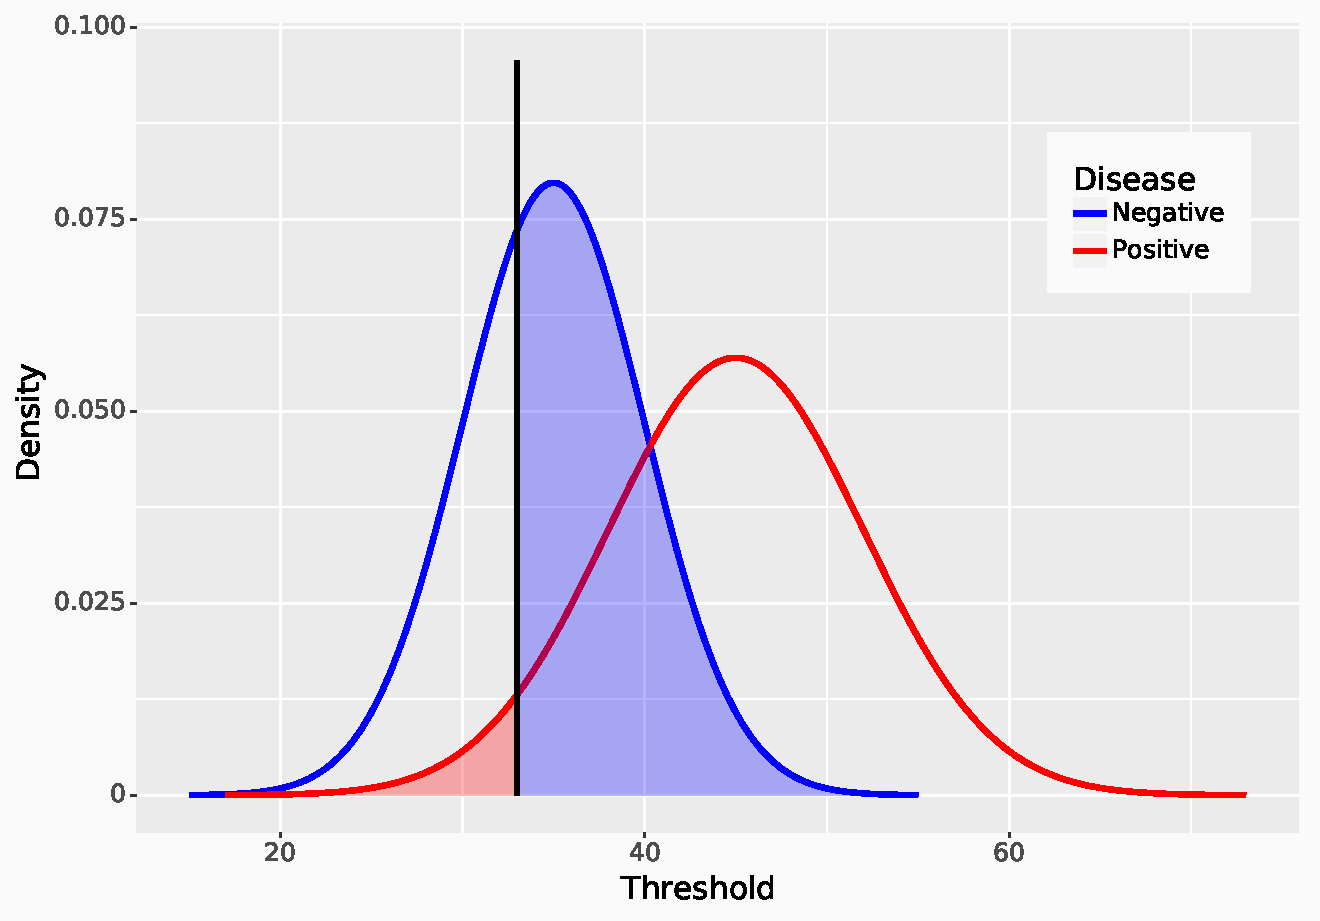
\includegraphics[height=0.45\textheight]{images/overlap_distr_tlow.pdf}\\
		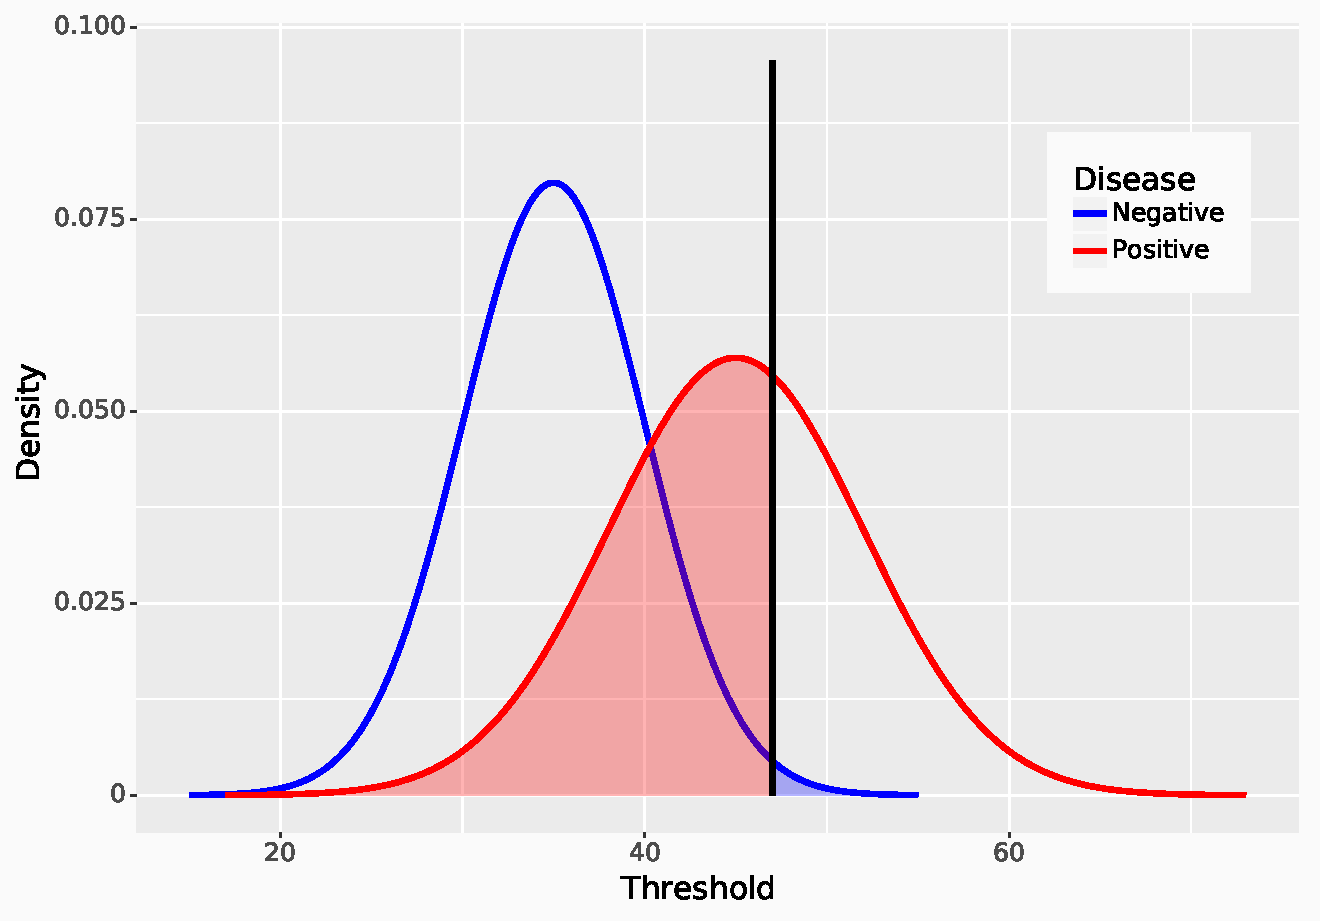
\includegraphics[height=0.45\textheight]{images/overlap_distr_thi.pdf}
	\end{center}
\end{frame}

\begin{frame}{Receiver Operating Characteristic}
	\begin{center}
		How can I evaluate a binary classifier over its range of possible discrimination thresholds?
	\end{center}
\end{frame}

%\begin{frame}
%	\begin{itemize}
%		\item Sensitivity = TP:FN (say everyone is positive)
%		\item Specificity = TN:FP (say everyone is negative)
%		\item PPV = TP:FP (high prevalence disease)
%		\item NPV = TN:FN (low prevalence disease)
%		\item Accuracy = (TP $+$ TN):(FP $+$ FN)
%	\end{itemize}
%
%\end{frame}


%F1 &= \frac{2 \times Sens \times PPV}{Sens + PPV} \\







\end{document}
